\section{需求分析}
\subsection{系统总体需求分析}
个人计算机和移动手机的存储不足是非常常见的现象,人们迫切地希望能有额外的空间对个人数据进行备份同时还可以方便地访问云端文件。
本系统的目的就是为了解决上诉用户的痛点,同时将闲置的网络和硬盘资源利用起来,起到积极的环保和省钱效果。整个系统具有下面的优点

\paragraph{完善的功能}本系统的个人网盘系统具有文件上传下载、公开分享、用户登录注册、视频在线播放、web端安卓端数据同步、手机文件自动
备份、文件标签、文件搜索、无线添加硬盘存储空间、文件操作符合用户平时在windows、安卓平台习惯的文件操作方式,用户可以没有学习成本就可以
使用本系统,本系统具有以上诸多优点。
\paragraph{先进的文件管理方法}本系统具有明确的管理方法,通过计算机网络技术为用户提供近乎无限的存储空间,解决用户数据丢失的担心,真正做到
方便好用的云盘系统。
\paragraph{成熟的技术}本系统基于主流的系统架构LAMP(Linux、Apache、Mysql、php)来开发,系统具有性能稳定、可扩展性高、安全可用等优点。
\paragraph{操作方便快捷}本系统提供web和安卓两种客户端访问方式,界面美观,操作逻辑符合用户习惯,用户无需特别学习,凭借之前在windows和安卓
平台积累的习惯就可以很快学会使用本系统。经过测试,在局域网的网络环境下,用户上传下载文件,在线视频都可以以接近网卡的速度进行服务器访问,
在广域网的网络环境下,本系统仍然可以提供基本的访问条件。
\paragraph{安全兼容性高}经过测试,本系统的web端在主流的浏览器Chrome、Edge、IE11、QQ浏览器、360安全浏览器、360极速浏览器、百度浏览器、
opera浏览器、手机端的uc浏览器、小米系统浏览器等浏览器都可以正常访问。同时系统的设计具有坚强的安全保密功能对用户个人信息进行保护,并提供
良好的接口,使得文件可以方便的导入导出。

\subsection{功能性需求分析}
在本章节中会介绍本系统所涉及到的功能需求,同时为了方便描述需求,引入了三种用户角色,一种是Web用户、一种是安卓用户、
另一种是非系统用户。非系统用户针对的是所有互联网用户,因为本系统涉及文件的分享,并且提供外网访问本地文件的方式,因此,作为
非本系统用户还是可以访问到系统用户分享后的文件的。

\subsubsection{用户控制需求}
在需求分析开始之初设计了两种注册方式和3种登录方式如下
\par 系统需要支持2种注册方式:
\par 1)账号;
\par 2)手机号,用户输入相应的注册信息完成注册。
\par 系统需要支持3种登录方式:
\par 1)通过账号登录;
\par 2)使用手机号直接登录;
\par 3)通过第三方平台登录,例如微信、QQ等。对于使用手机号登录。

但是在后期的开发过程中,发现注册和登录的功能并不是被系统所关键需要的,因为本系统的定位是局域网内家庭或者寝室成员之间交互,所以完全可以以纯
后端注册的方式来节省开发时间,因此在基于时间紧迫只实现了账号口令登录的功能。

如下用户用例图,web用户和安卓用户都可以进行登录、修改信息等操作,非系统用户不被赋予此项权限。
\begin{figure}[H]
  \centering
  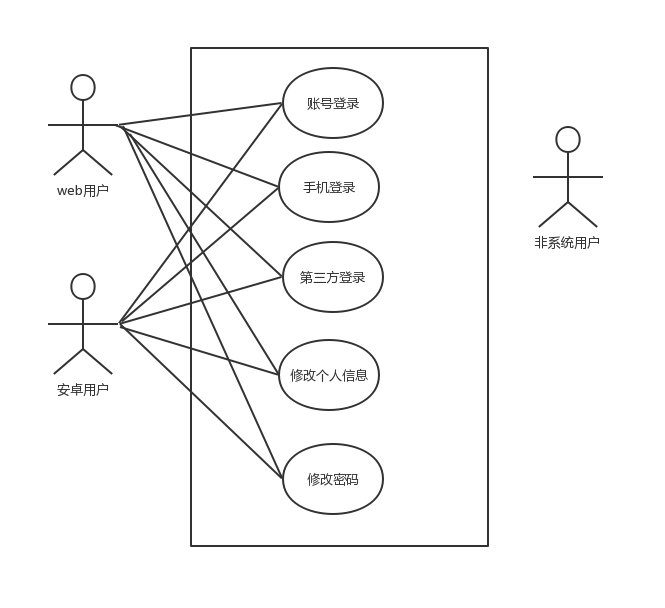
\includegraphics[width=80mm]{./figures/login_yongli.png}
  \caption{用户登录管理用例图}
\end{figure}

\subsubsection{文件/目录操作需求}
本系统提供云存储服务,自然有创建文件/目录、读写文件、删除文件/目录、访问文件/目录属性等。

如下用户用例图,

web用户存在文件上传、文件下载、或许文件详细信息、重命名文件、删除文件、查找文件、分享文件等需求。

安卓用户存在文件上传、文件下载、或许文件详细信息、重命名文件、删除文件、查找文件、分享文件等需求。

非系统用户可以访问下载被分享的文件,但是没有其他操作权限。

\begin{figure}[htbp]
  \centering
  \subfigure[文件管理用例图]{
  \begin{minipage}[t]{0.50\linewidth}
  \centering
  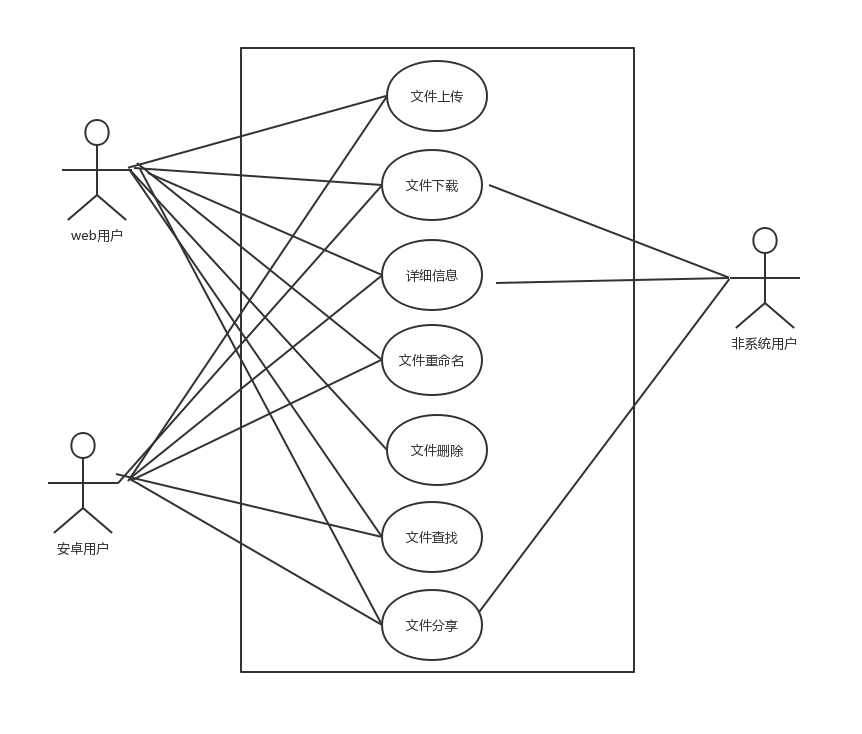
\includegraphics[width=65mm]{./figures/file_admin_yongli.png}
  %\caption{fig1}
  \end{minipage}%
  }%
  \subfigure[文件附加功能用例图]{
  \begin{minipage}[t]{0.50\linewidth}
  \centering
  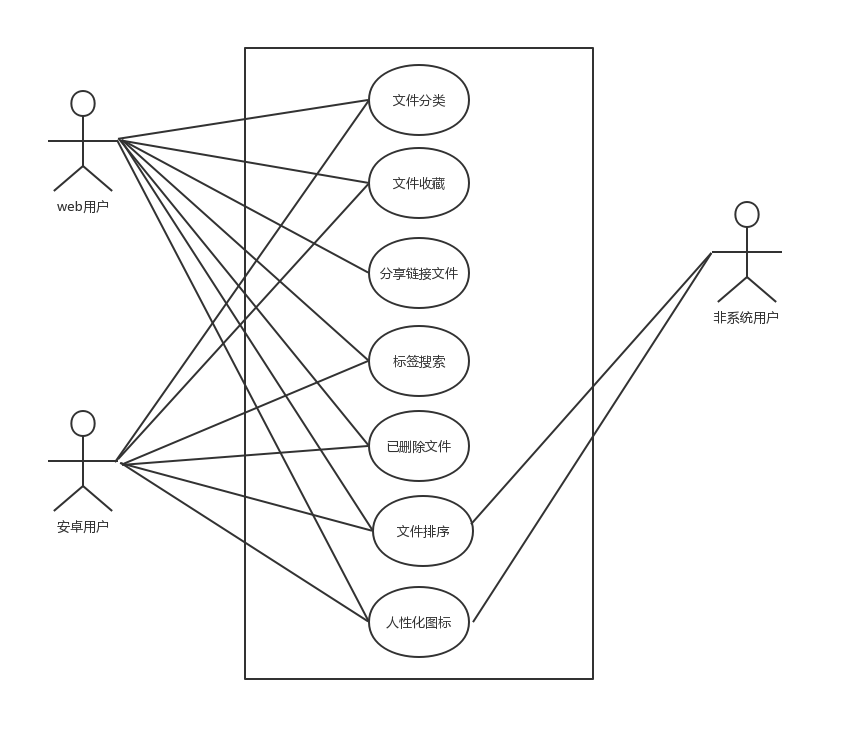
\includegraphics[width=65mm]{./figures/file_attach_yongli.png}
  %\caption{fig2}
  \end{minipage}%
  }%
  \centering
  \caption{文件操作用例图}
  \end{figure}
\subsubsection{文件/目录分享需求}
文件或目录分享是本系统一个非常重要的需求,市场上主流的云盘服务都有提供文件分享功能,同时为了系统安全考虑,
在实现系统的时候需要做一些安全性措施。

如下用户用例图,

web用户存在设置分享链接名称、设置分享密码、设置文件过期时间、修改分享信息、社交分享、访问下载分享文件等需求。

安卓用户存在设置分享链接名称、设置分享密码、设置文件过期时间、修改分享信息、社交分享、访问下载分享文件等需求。

非系统用户可以访问下载被分享的文件,但是没有其他操作权限。
\begin{figure}[H]
  \centering
  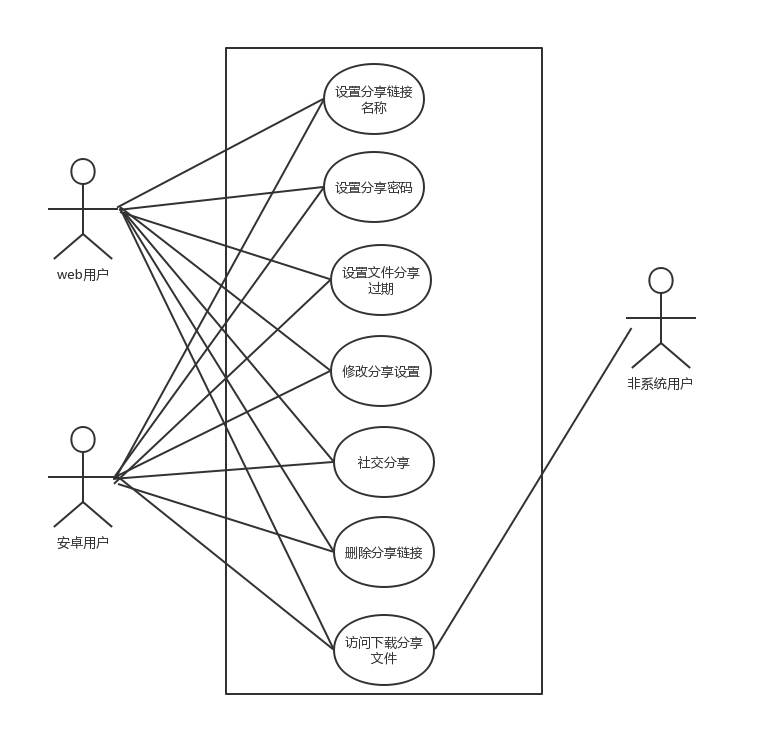
\includegraphics[width=120mm]{./figures/file_share_yongli.png}
  \caption{文件分享用例图}
\end{figure}

\subsubsection{视频在线播放需求}
视频和游戏、社交并称当今互联网三大主流需求,因此在线播放视频是本系统必须要实现的需求了。
本系统采用Apache作为服务器后端,对静态资源的访问有很好的支持,利用html5提供的video元素就可以很方便地实现
流媒体播放的功能,同时Apache对安卓端的VideoView也有很好的支持。

如下用户用例图,

web用户存在视频播放,图片预览、图片视频下载等需求。

安卓用户存在视频播放,图片预览、图片视频下载、图片自动备份、视频自动备份、WiFi环境上传文件、备份后删除原文件节省终端空间等需求。

非系统用户可以访问播放、预览、下载被分享的图片视频文件,但是没有其他操作权限。

\begin{figure}[H]
  \centering
  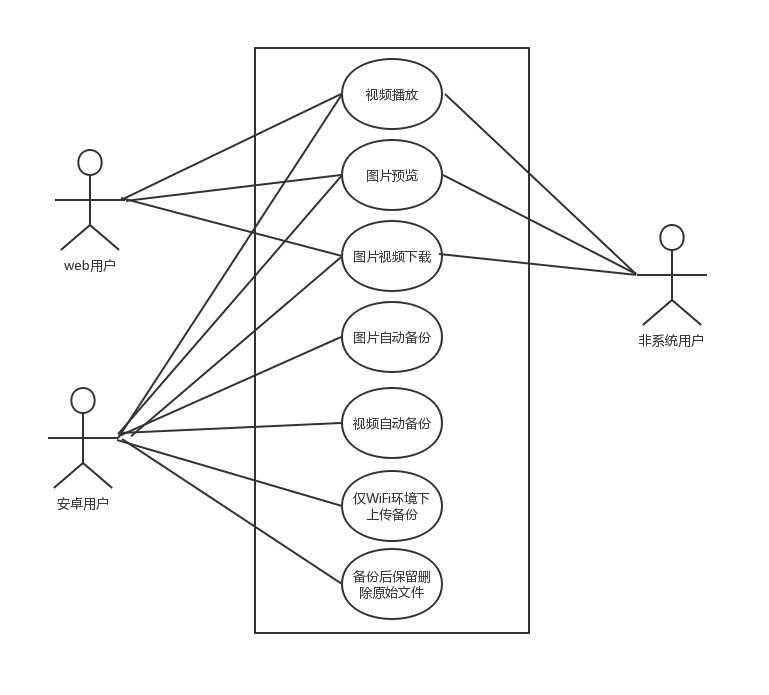
\includegraphics[width=130mm]{./figures/img_video_yongli.png}
  \caption{视频图片文件用例图}
\end{figure}

\subsection{非功能性需求分析}
\paragraph{响应时间} 
响应时间的定义是指一个客户端发送请求到服务器,然后接收服务器响应至结束的这一个过程中总共耗费的时间。响应时间包括三个部分,客户端呈现时间、网络传输时间和服务器响应时间。
其中客户端的呈现时间是指客户端在接收服务器返回的数据后然后渲染成可视化页面所消耗的时间,然后服务器的响应时间是指服务器从接收到客户端发来的请求,然后
在经过一些逻辑操作后(比如查询数据库,业务判断等)向客户端返回数据所消耗的时间。

本系统的使用场景一般位于局域网的环境下,响应时间需要做到基本处于2秒以下。同时如果处于外网的网络条件下,访问带宽也要达到中国电信所给予的500KB/S上载速度,
响应时间也需要做到5S以内。同时本系统是云盘系统,提供文件上传下载功能,因此网络的稳定性和速度都是重要的考量。其实就树莓派和路由器来说,网卡速度最大500Mb/s,因此
在软件算法上提升速度没有太大的意义,后期测试过程中,大文件的上传下载速度基本能保持在1.25MB/s左右的速度。

\paragraph{并发用户数}
并发的定义是多个用户在统一的时间点发送同一件事情或者操作的请求,这些操作一般都是相同的事务行为。
比如用户在互联网抢票的时候,会频繁的刷新结果,导致服务器不堪重负。再比如在文件上传的业务中,不同的用户可能上传相同名称的文件
并且在同一路径下,这时候就需要对该文件加锁才能保证后来的文件不会覆盖已有的文件了。同时,多个用户同时上传文件对孱弱的家庭宽带来说是
不小的挑战,因此并发量达到3个并发用户就可以满足本系统一开始的设定了。
  
\paragraph{吞吐量}
吞吐量的定义是指单位时间内系统接收并处理用户发起请求的数量,同时能够非常直观地体现服务器系统的性能承载力。
对于具有交互式性质的应用系统来说,吞吐量可以体现服务器系统所承受的性能压力。
在各种测试场景中,吞吐量一直都是一个重要指标,它可以在database、middleware和计算机硬件上得到直观的体现。
系统性能瓶颈可以用吞吐量来协助分析,还可以在设计软件性能测试场景用到吞吐量指标来衡量软件性能是否达到了预计的设计目标,
比如交互式应用系统中的Connection Pool、数据库事务发生频率、次数等。

\paragraph{资源利用率}
资源利用率是指对对计算机系统硬件和网络资源的利用程度,例如服务器的CPU利用率、内存利用率、磁盘利用率、网络利用率、GPU利用率等。
同时在改善系统性能的时候可以用资源利用率作为分析判断的重要指标。

在本系统的性能需求章,需要满足下列的性能指标。
\par(1)CPU使用率上限不超过百分之八十五
\par(2)内存利用率上限不超过百分之八十五
\par(3)磁盘I/O交换率上限不超过百分之八十五
\par(4)网络带宽平均可保持在1.25MB/s以上

\subsection{系统可行性分析}

\subsubsection{操作可行性分析}本系统的操作界面力求简洁明了,简化操作流程,使操作尽量符合用户的使用习惯和文件管理规范,用户无需特别学习就简单
上手,因此本系统的操作可行性是绝对可以的。
\subsubsection{技术可行性分型}
LAMP(Linux、Apache、MySQL、PHP)技术架构在世界范围内有非常广泛的应用,根据统计数据,世界上大约百分之七十2的网站都是基于LAMP
技术框架搭建。LAMP由Linux系统,Apache容器,Mysql数据库,PHP、Python等动态语言组成一个非常轻量和灵活的技术框架,开发环境的搭建也非常
方便,在github上有一键安装LAMP的脚本项目,受到世界上不少开发者的欢迎\cite{r27}。同时因为这个技术框架中所有组成产品均是开源软件,很多互联网企业的商业
应用都是采取这个架构,在开发成本和速度上有着明显的优势。J2EE也是开源产品,但是J2EE架构源、轻量、快速开发这些方面和LAMP相比处于劣势。
微软的 dot NET架构在通用、跨平台、性能、价格等方面也是明显不如LAMP架构,因此LAMP无论是性能、质量还是价格都是开发本云盘系统的第一选择\cite{r28,r29}。

本系统LAMP(Linux,Apache,Mysql,PHP)架构模式中,Linux基于Debian版本,具有稳定性强,升级方便,软件包丰富,性能优越,开发简单
等优点。同时采用Apache作为服务器,是因为Apache对静态资源的访问非常友好,避免了开发对静态资源的手动处理,大大节省了开发时间。
服务器规定了统一的API接口,无论是web客户端,还是手机APP客户端都可以采用统一的接口访问到服务器的资源,大大提升了开发效率。
同时数据库采用了开源的Mysql数据库,树莓派上Mysql版本是mariadb,相比于Oracle,MySQL具有开源免费,轻量易用,开发方便的优点,是互联网最流行的数据解决方案。
在本云盘系统中,所有用户信息、文件路径信息、分享文件信息、系统配置信息和其他类型的信息都存储于数据库中,通过SQL语言可以很容易地查询这些信息。PHP是开源的动态语言,它既可以用来做后台业务逻辑的开发,
也可以嵌入到HTML中实现前端效果,也可以访问MySQL数据库中的数据和 Linux 提供的一些特性的动态内容。因此PHP非常适合web开发和为Android数据访问提供接口。
同时因为服务器是部署在中国电信给予的局域网内,所以如果需要外网访问,就需要进行端口映射,端口映射的时候要避免将外网端口设置成常见的80端口,
因为中国电信会为了网路安全,对特定端口不允与开放。同时系统后台会开放一个备份进程,定时对文件进行备份。
\newpage
